\chapter{自相位调制}
\label{ch:SPM}

在具有三阶非线性的材料中,某一时刻的折射率取决于该时刻的光功率。因此,与低功率但形状相同的脉冲相比,高功率脉冲将经历更大的相位变化。由于非线性介质中可以同时存在不同频率的光,描述非线性对光场的影响可能较为复杂。本章解释了一个简单的情况,即“自相位调制”(SPM),其中仅存在一个以单一载频为中心的脉冲。

\section{脉冲中的相位变化}
从方程~\ref{eq:GNLSE}出发,并假设除$\gamma>0$之外的所有参数都为零,$\omega_0\A\gg\partial_T\A$,且$R(T_{delay})=\delta(T_{delay})$,则广义非线性薛定谔方程简化为
\begin{align}
\label{eq:SPM}
    \partial_z\A &= i\gamma|\A|^2\A.
\end{align}
从数学角度看,方程~\ref{eq:SPM}表明,对于$z$的微小变化,复数$\A$的变化量等于其自身在复平面上旋转90度($i\A$),并根据其自身的平方模($|\A|^2$)以及标量$\gamma$进行缩放。从物理角度看,方程~\ref{eq:SPM}暗示非线性效应会根据功率改变场的瞬时相位,但不会改变该瞬时的功率大小。解方程~\ref{eq:SPM}得到
\begin{align}
    \label{eq:SPM_applied}
    \A(z,T)&= \A(0,T)\exp\left( i\gamma|\A(0,T)|^2z \right).
\end{align}
为了理解方程~\ref{eq:SPM_applied}的含义,可以参考方程~\ref{eq:chirp_definition},该方程指出脉冲的瞬时频率与其相位相对于时间的负导数有关。假设一个高斯脉冲$\A(0,T)=\A_0\exp(-T^2/2T_0^2)$,则该脉冲在通过非线性介质传播距离$z$后的瞬时频率为
\begin{align}
\label{eq:SPM_example}
    \delta\omega(z,T) &= -\gamma |\A_0|^2 z\partial_T \exp\left(-\frac{T^2}{T_0^2}\right)\\ \nonumber
    &= 2\gamma |\A_0|^2 z T/T_0^2 \exp\left(-\frac{T^2}{T_0^2}\right),
\end{align}
这表明脉冲前沿将产生红移,后沿将产生蓝移。参见图~\ref{fig:chirp_profiles}(a)以了解高斯脉冲产生的啁啾可视化,参见图~\ref{fig:chirp_profiles}(b-d)以了解其他脉冲形状产生的啁啾。考虑方程~\ref{eq:SPM_applied}中指数的参数,可定义非线性效应变得显著的特征长度为
\begin{align}
    L_{NL} &= \frac{1}{\gamma P_0} = \frac{1}{\gamma |\A(0,T)|^2},  
\end{align}
其中$P_0$为脉冲的初始峰值功率。

\begin{figure}
    \centering
    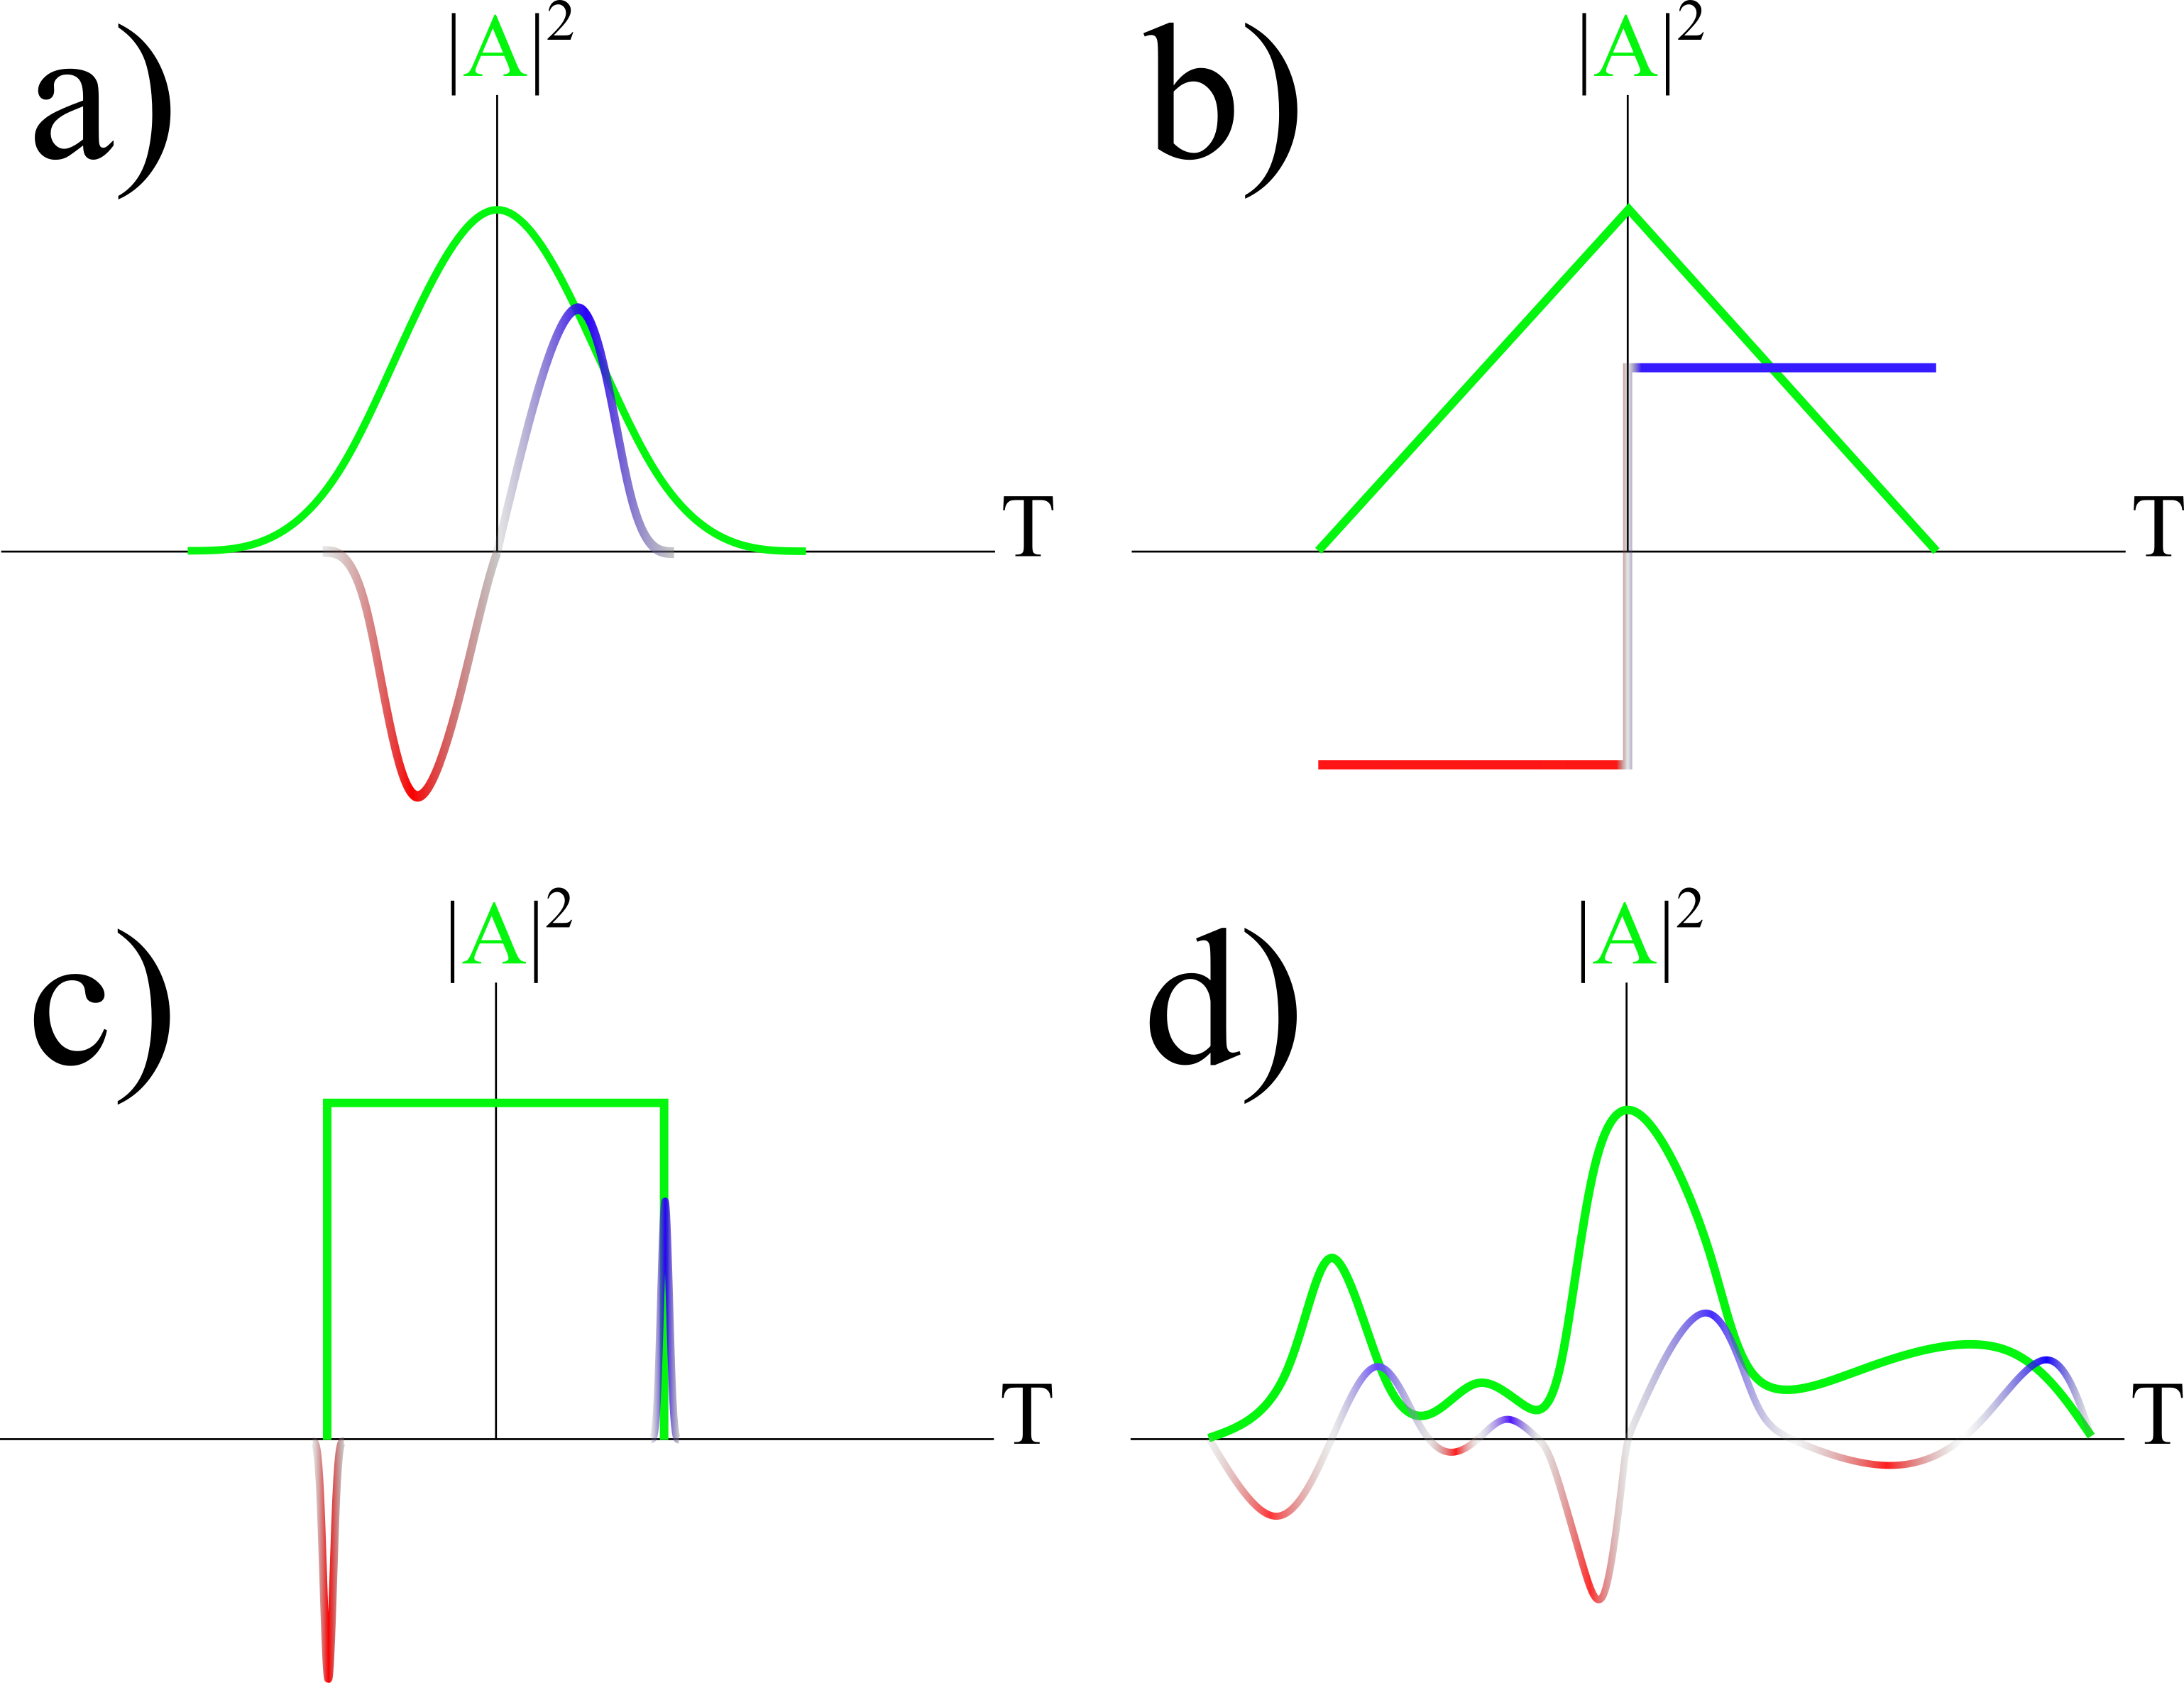
\includegraphics[width=0.75\linewidth]{figures/SPM_chirp.png}
    \caption{SPM对(a)高斯脉冲,(b)三角脉冲,(c)方波脉冲,(d)任意脉冲的影响可视化。一般来说,正斜率会导致红移啁啾,负斜率导致蓝移啁啾,水平斜率则不会产生啁啾。}
    \label{fig:chirp_profiles}
\end{figure}

\section{谱展宽}
对等式~\ref{eq:SPM_example}的分析表明,自相位调制(SPM)会导致脉冲在前导坡度上变得“更红”,在后导坡度上变得“更蓝”。单独考虑时,$\betag_2>0$也会导致类似的行为,但关键区别在于,色散仅改变不同频率分量的相对相位,而SPM还会改变它们的幅度。换句话说,作用在脉冲上的SPM会产生新的颜色,这些颜色在最初并不存在!通过对等式~\ref{eq:SPM}两边进行傅里叶变换可以从数学上看到,这意味着在频谱域中的展宽,因为傅里叶变换在时域中两个函数的乘积等效于频域中的卷积:

\begin{align}
\label{eq:SPM_freq}
    \partial_z\Tilde{\A} &= i\gamma \FT\left\{\A\A^*\A\right\} \\ \nonumber
    &= i\gamma \Tilde{\A}*\Tilde{\A^*}*\Tilde{\A}.
\end{align}

简而言之,等式~\ref{eq:SPM_freq} 表明 $\A$ 的频谱相对于 $z$ 的变化取决于其频谱与自身及其复共轭的卷积。由于卷积两个函数会产生一个比初始函数更宽的函数,等式~\ref{eq:SPM_freq}显示频谱将随距离的增加而展宽,暗示通过将功率从载波向红、蓝端转移而添加新频率。请参见图~\ref{fig:SPM_before_and_after},了解SPM对高斯脉冲的影响示例。

\begin{figure}
    \centering
    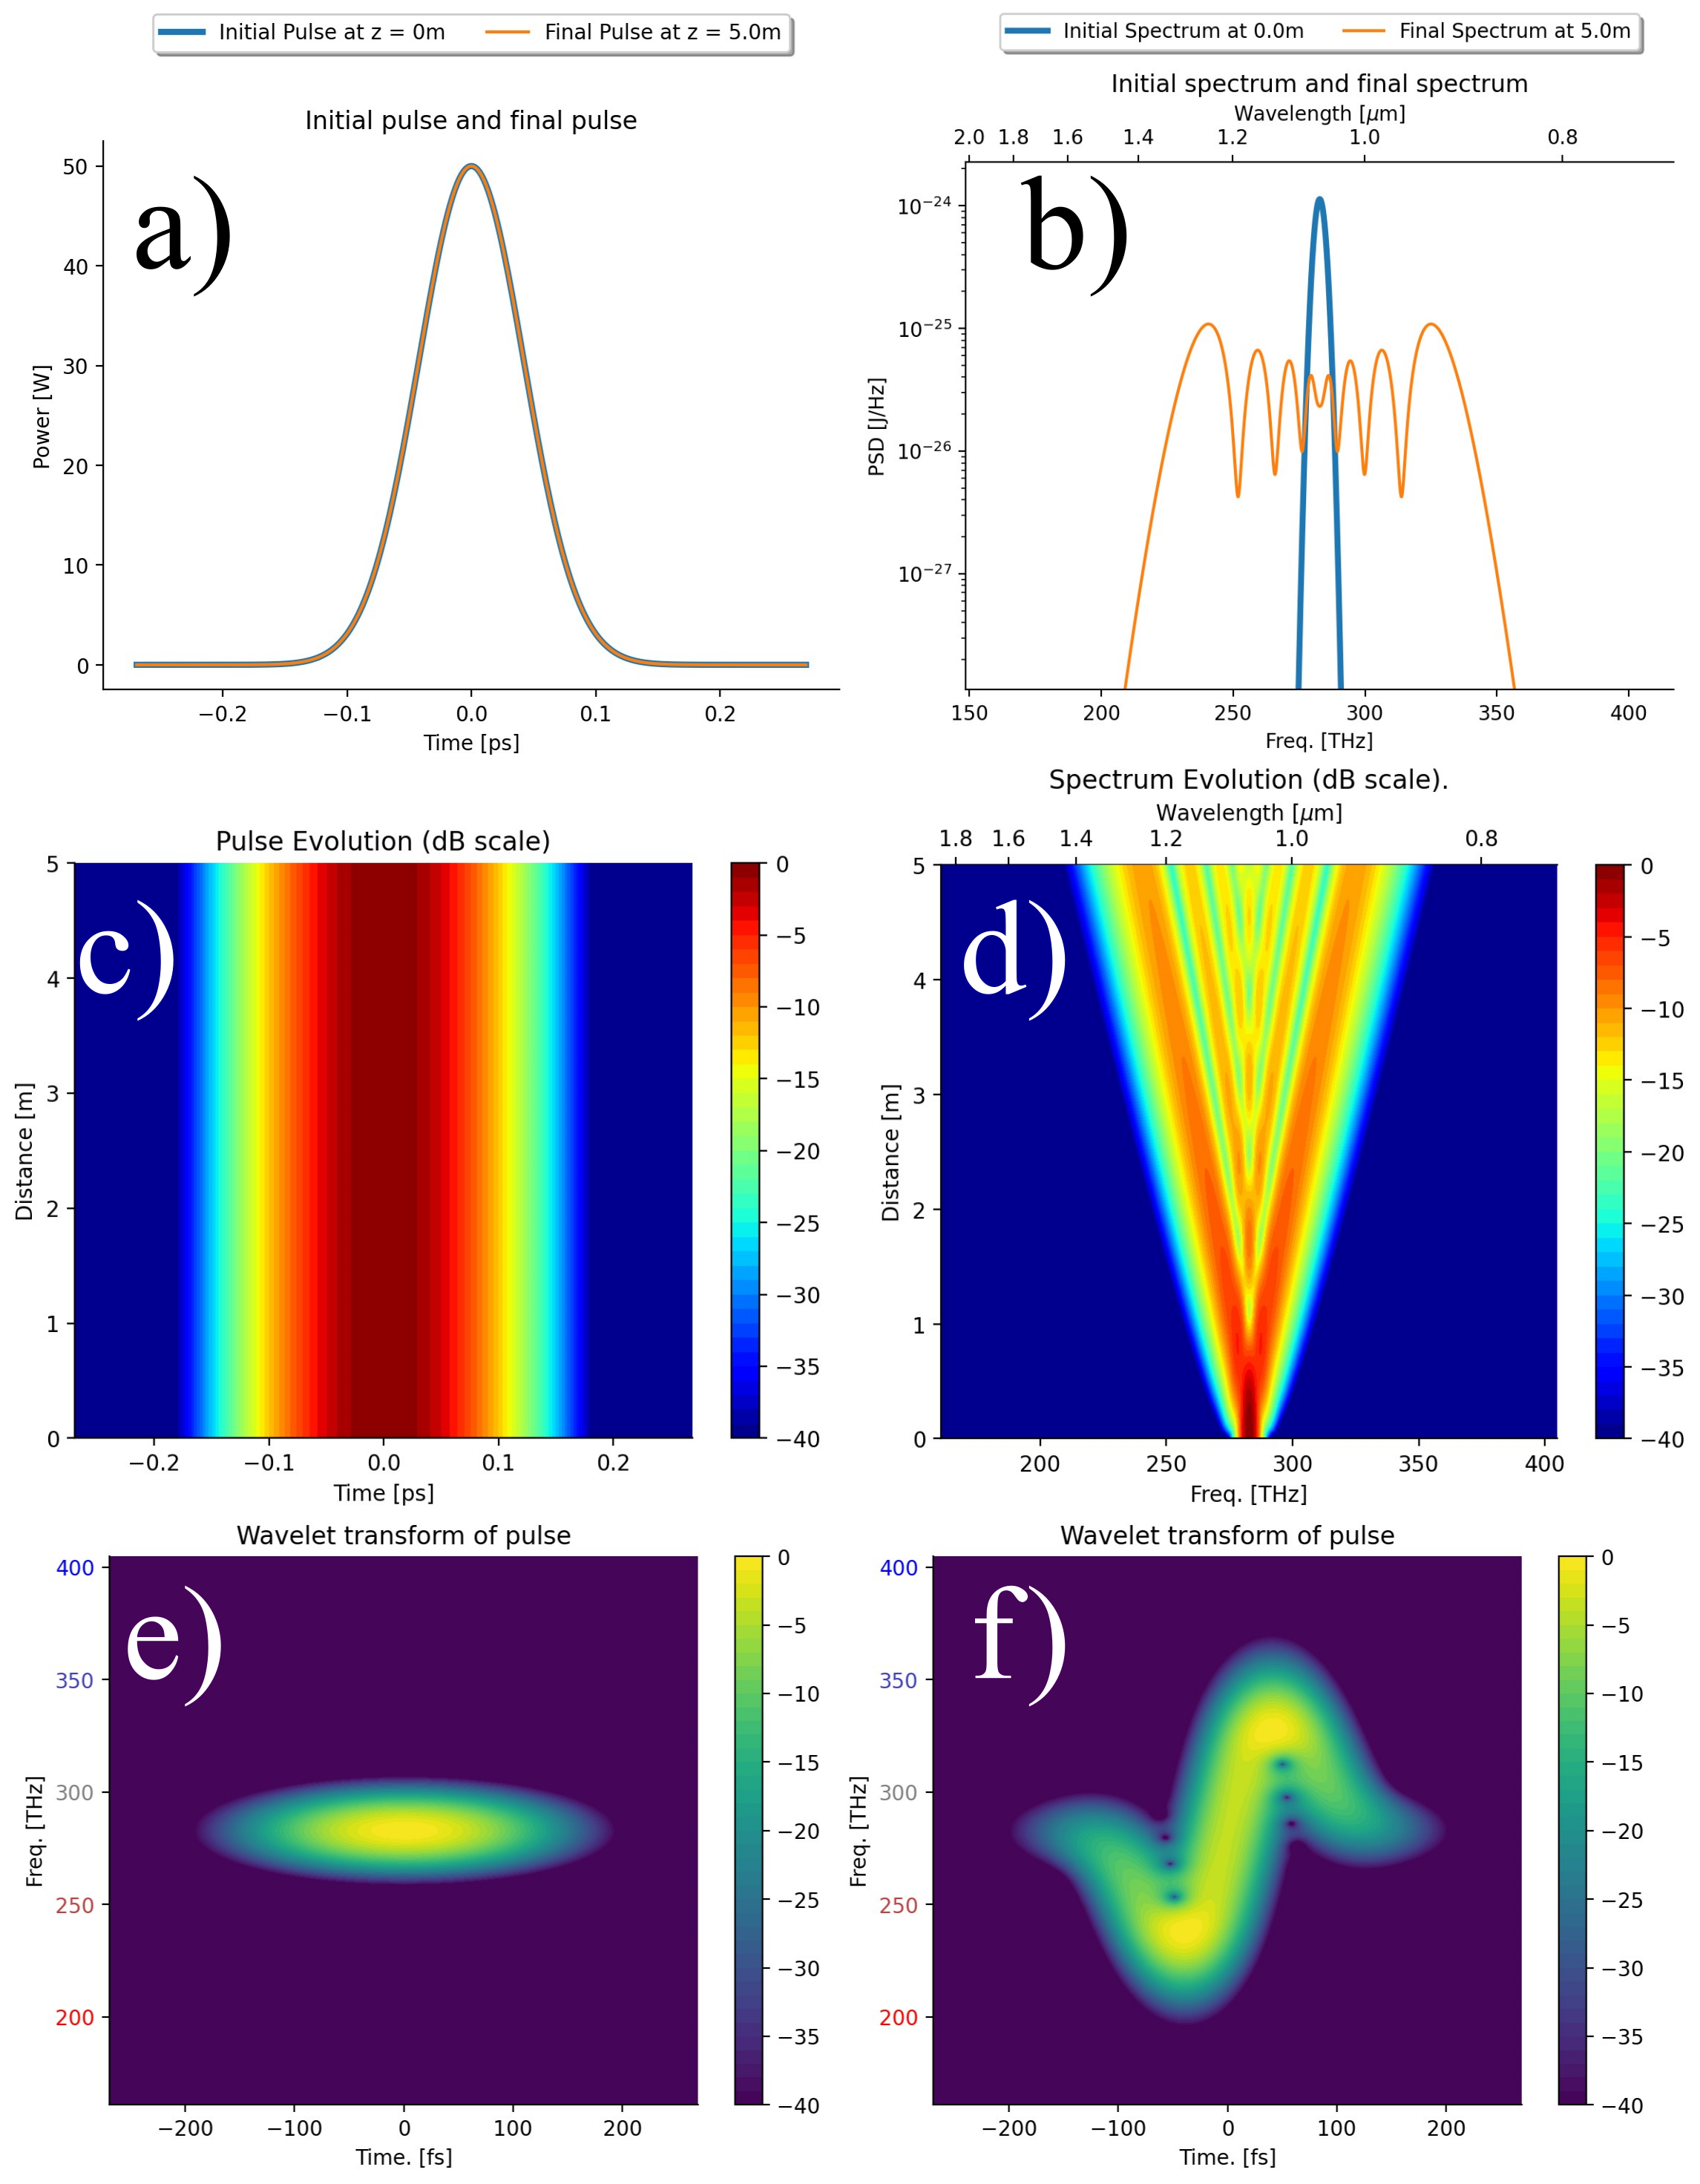
\includegraphics[width=1\linewidth]{figures/SPM_combined.png}
    \caption{ 高斯脉冲在由等式~\ref{eq:SPM}描述的非线性介质中传播的前后对比。
    a) 在时域中,脉冲的功率包络保持不变。 b) 频谱展宽。 c) 时域中功率包络的演化没有变化。 d) 频谱逐渐展宽。 e) 传播前的脉冲频谱图。 f) 传播后的脉冲频谱图。请注意频谱域中的展宽以及时间域中宽度的恒定。使用\href{https://colab.research.google.com/drive/1P41F4hO6Mv12RsEkpogYv5teQyFZ6iW0?usp=sharing}{这个交互notebook}中的数值模拟生成图形,读者可以尝试进行实验。}
    \label{fig:SPM_before_and_after}
\end{figure}


\section{自相位调制、损耗与“有效长度”}
考虑等式~\ref{eq:GNLSE},假设与等式~\ref{eq:SPM}相同,但此时 $\alpha\neq0$。回忆等式~\ref{eq:attenuation_power},其中 $\alpha\neq0$ 会导致脉冲功率随距离呈指数变化。在这种情况下,

\begin{align}
\label{eq:SPM_and_loss}
    \partial_z\A &= \frac{\alpha}{2}\A +i\gamma|\A|^2\A\\ \nonumber
    &=\left(\frac{\alpha}{2} +i\gamma |\A(0,T)|^2 \exp(\alpha z) \right)\A. 
\end{align}

将等式~\ref{eq:SPM_and_loss} 从 $0$ 积分到 $z$ 得到:

\begin{align}
    \label{eq:Leff_derivation}
    \A(z,T)&=\A(0,T) \exp\left( \frac{\alpha}{2}z+i\gamma|\A(0,T)|^2 \int_0^z \exp(\alpha\xi) d\xi  \right) \\ \nonumber
    &=\A(0,T) \exp\left( \frac{\alpha}{2}z+i\gamma|\A(0,T)|^2  \frac{\exp(\alpha z)-1}{\alpha}   \right) \\ \nonumber
    \A(L,T)&=\A(0,T) \exp\left( \frac{\alpha}{2}z+i\gamma|\A(0,T)|^2  L_{eff}   \right),
\end{align}

其中,具有实际长度 $L$ 的介质的“有效长度”定义为:

\begin{align}
\label{eq:L_eff}
    L_{eff}= \frac{\exp(\alpha L)-1}{\alpha}.
\end{align}

等式~\ref{eq:Leff_derivation} 和等式~\ref{eq:L_eff}提供的见解是,尽管通过让光在更长的介质中传播通常会增强非线性效应,但该介质的损耗最终会使光功率降低到所有非线性效应变得可以忽略的程度。例如,对于典型的100公里长单模光纤(损耗系数为$\alpha=-0.22$dB/km),其有效长度约为19.6公里。换句话说,光信号在100公里有损耗光纤中的非线性相移累积量大致等于在19.6公里无损耗光纤中的累积量。请参见\href{https://www.desmos.com/calculator/g6dadbxq33}{这个互动图表}以查看有效长度如何依赖于 $\alpha$。注意,当 $\alpha L\ll 1$ 时,$L_{eff}\approx L$;而在 $\alpha>0$ 的情况下(如在光放大器中),可能出现 $L_{eff}>L$。此外,$\alpha$ 在特殊的非均匀光纤或存在拉曼放大时可能随 $z$ 而变化,此时需要相应修改等式~\ref{eq:attenuation} 和等式~\ref{eq:SPM_and_loss}。

\section{自陡效应}
\label{sec:SS}

在等式~\ref{eq:SPM}中,假设非线性相位偏移与场包络乘以其平均功率成正比,即 $\A|\A|^2$。这种假设可以视为非线性响应的相对于时间的零阶泰勒近似,类似于将 $\exp(x)\approx 1$ 用于非常小的 $x$。若进一步假设场包络的变化率乘以其平均功率 $\partial_T(\A|\A|^2)$ 也有贡献,则得到:

\begin{align}
\label{eq:SS}
    \partial_z\A &= i\gamma\left(1+\frac{i}{\omega_0}\partial_T \right)\A|\A|^2.
\end{align}

在等式~\ref{eq:SS}中的括号内,第一个项是自相位调制(SPM),而第二个项称为“自陡效应”(SS)。物理上,可以理解为非线性效应导致脉冲高功率部分的折射率发生显著变化。较高的折射率意味着光传播速度更慢,因此高功率脉冲的峰值在传播时比较低强度部分减速,从而在后续时间上积累功率,导致坡度陡降。类似地,一辆大且不流线型的卡车在遇到强逆风时会比流线型汽车大幅减速,从而在后方形成堵塞,而前方交通则较稀疏。由于SS效应平坦化了脉冲前端的功率坡度,并使后端变得陡峭,因此优先将脉冲频谱蓝移,因为 $\delta\omega\propto -\partial_T|\A|^2$。请参见图~\ref{fig:SS},了解SS对与图~\ref{fig:SPM_before_and_after}相同高斯脉冲的影响。对于仅受SPM和自陡效应影响的高斯脉冲,\href{https://prefetch.eu/know/concept/self-steepening/}{可以证明}其后坡在距离

\begin{align}
    L_{SS} &= \frac{T_0\omega_0\exp(1/2)}{3\sqrt{2}\gamma P_0}
\end{align}

处变得无限陡。

更多关于SS的信息,请参考\href{https://youtu.be/Fr6yLtGZ2To}{这个视频教程}。

\begin{figure}
    \centering
    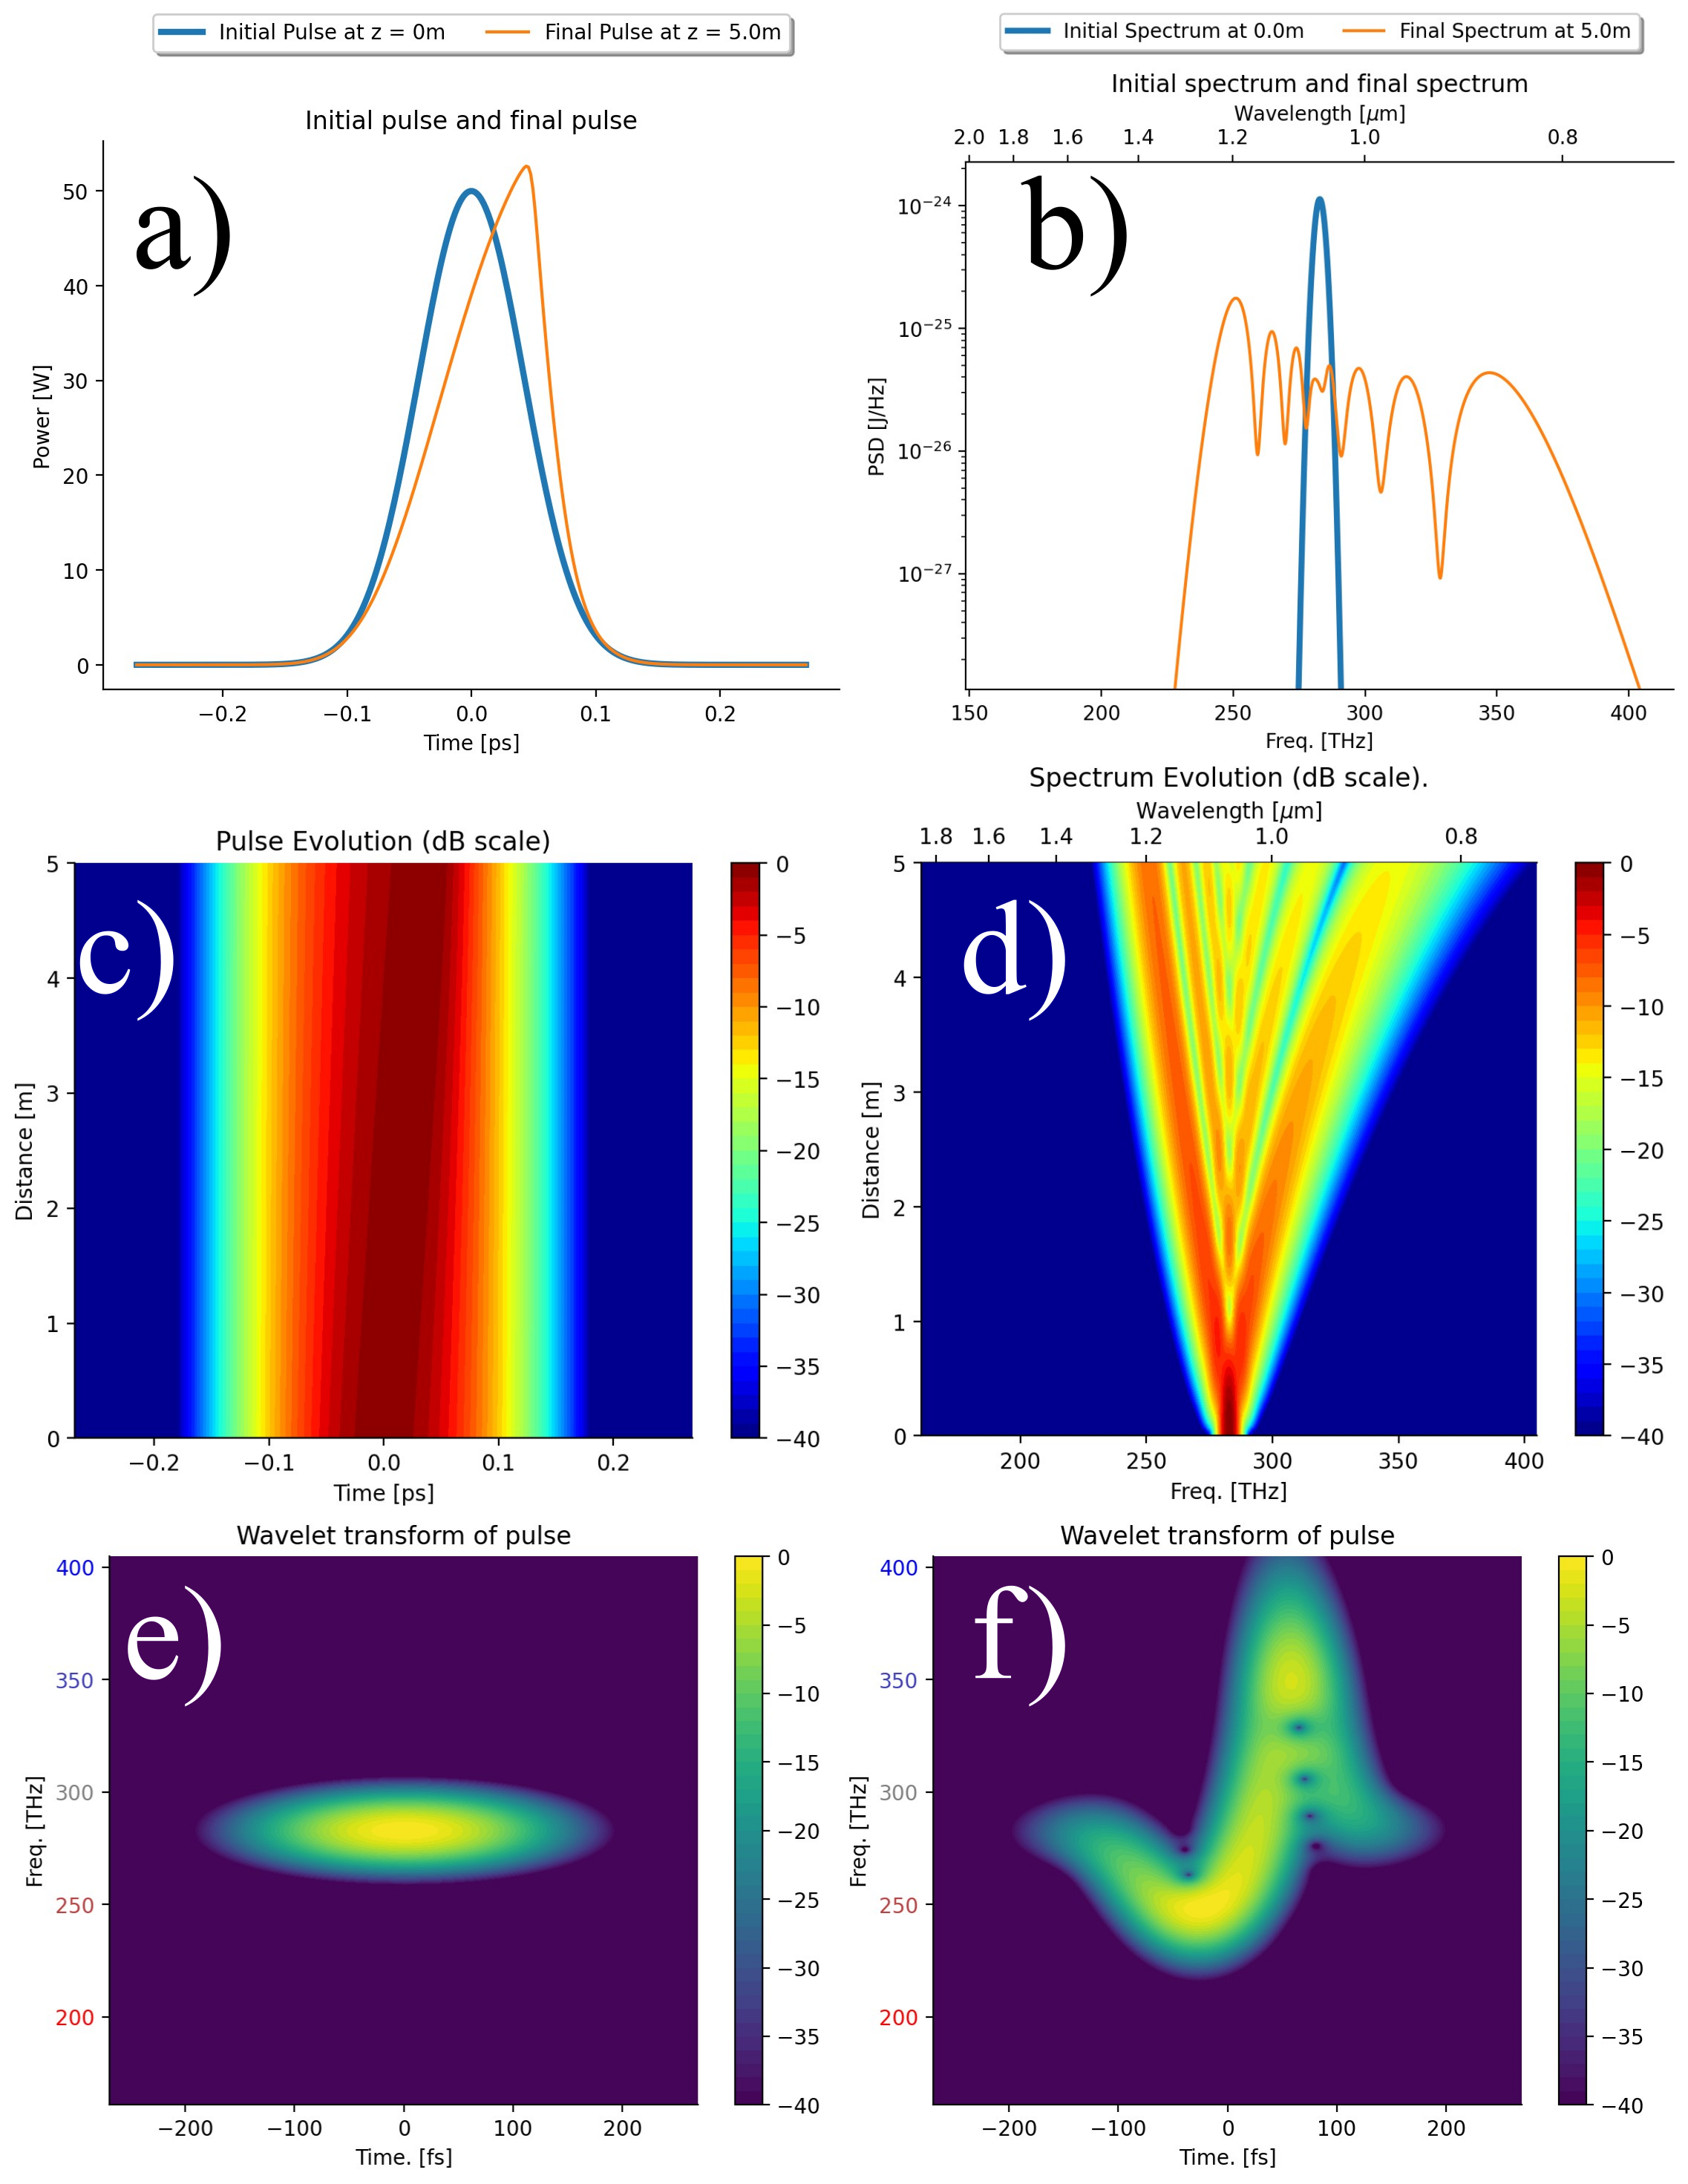
\includegraphics[width=1.0\linewidth]{figures/SPM_and_SS_combined.png}
    \caption{高斯脉冲在由等式~\ref{eq:SS}描述的非线性介质中传播的前后对比。 
    a) 在时域中,脉冲的功率包络在后端变得更陡,因为非线性效应导致脉冲峰值处的折射率较高并减速。 b) 频谱由于后端的陡降坡度向更高频率不对称展宽。 c) 时域中功率包络的演化。 d) 频谱逐渐向高频展宽。 e) 传播前的脉冲频谱图。 f) 传播后的脉冲频谱图。使用\href{https://colab.research.google.com/drive/1P41F4hO6Mv12RsEkpogYv5teQyFZ6iW0?usp=sharing}{这个交互notebook}中的数值模拟生成图形,读者可以尝试进行实验。}
    \label{fig:SS}
\end{figure}

\subsection{适用性}
由于SS的影响与 $\omega_0\approx 2\pi/200~\text{THz} = 2\pi/5$fs 成反比,且对于长脉冲 $\A|\A|^2$ 的时间导数较小,SS效应在脉宽低于100~fs时较为显著,在数百fs量级的脉宽时较为显著,而对于超过几ps的脉宽则可忽略不计。



